{\bf BME154L - Exam \#1}\hfill Name:\underline{\hspace*{3.0in}}



\section{[20 points]}

Impedances can be in terms of $R$s and $C_1$.  Please don't answer the `Why?' questions below with more than 2-3 sentences!!

\begin{center}
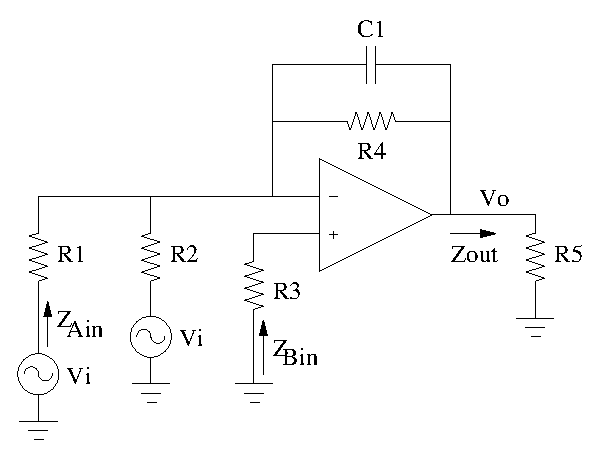
\includegraphics[width=3.0in]{zin_zout}
\end{center}

\begin{enumerate}
\item What is the input impedance ($Z_{A_{in}}$), as indicated on the circuit above?
\vspace*{0.5in}
\item What is the input impedance ($Z_{B_{in}}$), as indicated on the circuit above?
\vspace*{0.5in}
\item Which input impedance is more ideal when working with voltage input signals?  Why?
\vspace*{1.0in}
\item What is the output impedance ($Z_{out}$), as indicated on the circuit above?
\vspace*{0.5in}
\item What is the ideal output impedance when working with voltage signals?  Why?
\end{enumerate}


\clearpage
